
\chapter{融合统计机器翻译技术的中文输入方法}
\label{Chapter_cocat}

计算机辅助翻译被广泛用于帮助和管理人工翻译过程,其核心思想是利用翻译记忆提升生产效率。如果能从翻译记忆中找到与当前句子匹配程度较高的句对,则仅需要非常少的工作量就能较好地完成翻译任务。但在大部分情况下,待翻译句子和翻译记忆的匹配程度并不高。因此,随着机器翻译译文质量的不断提高,人们希望通过引入机器翻译来进一步提高人工翻译效率。译后编辑是目前将机器翻译应用于人工翻译的最佳实践,即直接将自动译文修改为满足要求的最终译文。如果机器翻译的自动译文质量较高,人工修改量就比较少,因而这种方式可以有效提升译员的生产效率。

然而在行业实践中,译后编辑面临诸多现实挑战。主要原因是当前的机器翻译系统对应的译文质量远未达到人工翻译场景中专业译员的期望。如果机器翻译的自动译文质量较差,译员不得不分析和修改漏洞百出的自动译文,其代价甚至可能超过直接翻译。僵化的译文和似是而非的术语翻译使得译员使用机器翻译的热情并不高,而重复纠正错误的乏味感和反复修改仍不能满意的挫败感也使译后编辑的译员感到沮丧。虽然近两年来,神经网络机器翻译发展迅猛,译文质量显著提升,但仍需要相当长时间才可能在实践中显著改善译后编辑的人机交互体验。
结合实际的人工翻译过程,通过分析我们发现,一般在自动译文中总能找到可以直接使用的完美片断。因此,就目前的技术条件而言,我们认为最重要的是以尽可能简单的方式,充分利用机器翻译结果中的正确部分,同时应该尽量避免让译员受到错误部分的干扰。

为了达到这个目的,我们在本章提出一种融合统计机器翻译技术的中文输入方法。该输入方法面向人工翻译场景,根据用户按键,将统计翻译中的翻译规则、翻译假设列表和n-best列表等相关信息融合进输入方法,只需较少的按键次数就可以生成准确的译文结果。使用该输入法,译员可以完全不阅读机器翻译的自动译文,但仍可以得到机器翻译的帮助。因此,相对译后编辑而言,即使机器翻译自动译文的质量较低,该输入法也能显著改善译员的人机交互体验。此外,为了指导统计机器翻译系统生成更适合输入方法的翻译结果,我们提出了面向输入方法的机器翻译译文自动评价指标,使该输入方法利用更合适的统计翻译结果,进一步提升人工翻译效率。

本章的组织结构如下:3.1节介绍基于对数线性模型的中文拼音输入方法,然后在3.2节中讨论输入一个汉字需要按多少键;3.3节详细介绍融合统计机器翻译技术的输入方法;3.4节提出了面向输入方法的译文自动评价指标;3.5节介绍了已有相关工作;3.6节给出详细的实验结果和分析,最后的3.7节对本章进行总结。

\section{基于对数线性模型的输入方法}

输入法用于输入中文或其他大型形意文字,比如超过97\%的中文用户使用拼音输入法输入汉字[\cite{chen:1997}]。汉字的输入过程本身就是人机交互过程。为简洁起见,如无特别说明,下文均以拼音输入法为例。输入法输入汉字的快慢不仅取决于对汉字编码的平均长度,即击键次数,还取决于寻找按键所需要的时间。例如,相对于用户选择的全拼输入法而言,双拼输入法中每个声母和韵母只用一个键表示,看似节省了一点击键次数,但是输入并不快,而且学习也很困难。发展的结果是拼音输入法一般指全拼输入法。所以,改进输入法时,除了优化编码长度,还要注意兼顾自然流畅的人机交互体验。

拼音输入法的解码过程是将用户输入的拼音音节串转换成对应汉字串的过程。中文共有405个音节,如zi(自)、ran(然)、yu(语)、yan(言)等等,而常用简体中文字符集GB2312中包含6763个常用汉字。此外,用户希望仅输入音节的前缀就能得到正确的结果,如更倾向于通过输入“zryy”而得到“自然语言”。因此,每一个音节或者前缀可以对应多个汉字,拼音输入法必须解决重码率较高的问题。为简洁起见,后文我们将一个音节或者它的前缀笼统地称为“拼音”,如“ziranyuyan”和“zryy”都包含四个拼音。

\begin{figure}[!tb]
	\centering
	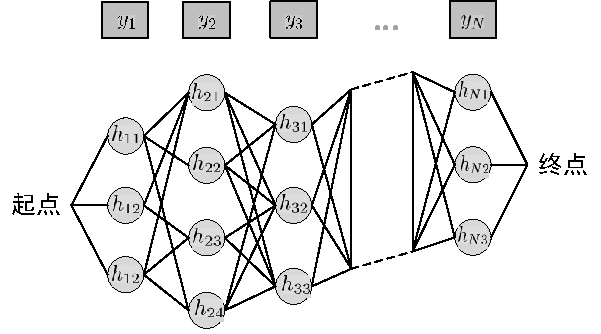
\includegraphics[width=0.88\textwidth]{Figure/Figure_3_1.pdf}
	\caption{拼音到汉字转换解码的网格图}
	\label{Fig_pinyin_to_character}
\end{figure}

每个拼音对应多个汉字,把一个拼音串对应的汉字从左到右连起来,就是一张如图\ref{Fig_pinyin_to_character}所示的网格图。$y_1,y_2,y_3,\ldots,y_N$是用户输入的拼音串,$N$为拼音数,也是输入法短语候选的汉字数;$h_{11},h_{12},h_{13}$是第一个拼音$y_1$的候选汉字(在后文中,我们用变量$h_1$代表这三个候选字);$h_{21},h_{22},h_{23}$是对应于拼音$y_2$的候选汉字,以变量$y_2$统一代表,以此类推。从第一个字到最后一个字可以组成很多句子,每一个句子和图中的一条路径一一对应。拼音输入法就是要根据上下文在给定拼音条件下找到一个最优的输入短语,我们利用对数线性模型可以形式化为:
\begin{equation}
\label{input_method_linear}
\widehat{H}(y_1^n) =  \argmax_H \sum_{m=1}^{M} \lambda_m f_m(h_1^n, y_1^n)
\end{equation}
其中,$h$为输入结果,$\lambda_m$为对应特征函数的权重,$M$为特征函数的个数。一般而言,拼音输入法包括以下典型特征函数:

(1)音字转换概率;

(2)字音转换概率;

(3)语言模型概率;

(4)输入法短语候选中各词的使用概率;

(5)输入法短语候选的使用概率;

(6)在短期输入历史中,输入法短语候选中的各词的命中概率;

(7)在短期输入历史中,输入法短语候选的命中概率。

\section{输入一个汉字需要按多少键}

假设某输入法的输入能力为常用简体中文字符集GB2312中包含的6763个常用汉字,且只能用键盘上的26个英文字母对汉字进行编码。假设每个汉字出现的相对频率为$p_1,p_2,p_3,\ldots,p_{6763}$,编码的长度为$l_1,l_2,l_3,\ldots,l_{6763}$,则汉字的平均编码长度为:

$L = p_1 \times l_1 + p_2 \times l_2 + p_3 \times l_3 + \ldots + p_{6763} \times l_{6763}$.

\noindent汉字的信息熵为:

$H = -p_1 \times \log p_1 + p_2 \times \log p_2 + p_3 \times \log p_3  + \ldots + p_{6763} \times \log p_{6763}$

参考文献[\cite{wujun:2012}]的计算过程,由香农第一定理,任何信息编码的长度都不小于它的信息熵,则可以得出:

$L \ge H$

根据文献[\cite{feng:1984}]的计算结果,一个汉字的熵为9.65比特,也就是10比特以内。即便进一步扩大汉字容量,这个熵值也不会再增加。因此,键盘上的每个字母可以代表$\log_2 26 \approx 4.7$比特信息。

综上所述,输入一个汉字的平均按键数为$9.65/4.7 \approx 2.1$。
在本章中,我们认为输入一个汉字的平均按键次数的理论下限值为2。根据香农第一定理,如果把汉字组成词,即编码的基本单位为词,则每个汉字的平均信息熵会减少至8比特左右,即输入一个字的平均按键数为1.7。如果再考虑上下文相关性,如引入统计语言模型,可以将汉字的平均按键数降至1.3。其它语言文字输入方法的相关讨论,可参见文献[\cite{Garay-Vitoria:2006}]。

但是,目前还没有一种输入法能接近如此高的输入效率。首先,只有对汉字的词组根据词频进行特殊编码才能接近理论极限,这样反而会造成看似节省了一点按键次数,但是输入并不快的结果。其次,由于输入法软件运行环境的计算资源的受限,我们不可能利用特别大的语言模型或者其它特别依赖计算资源的上下文信息。实际上,在兼顾人机交互体验的情况下,如果拼音输入法达到每个汉字的平均按键次数为3.7就比较成功了[\cite{Cui:1985}]。如果能够更多地利用上下文相关性,文献[\cite{wujun:2012}]认为拼音输入法的平均按键次数小于3就很优秀了。

\section{融合统计机器翻译技术的输入方法}

以如下英语到汉语的翻译任务为例:

\begin{center}
	\begin{boxedminipage}[h]{0.85\linewidth}
		源语言句子$s$:
		
		\quad \quad China mulls change to officials' welfare system
		
		机器翻译自动译文MT:
		
		\quad \quad 中国 考虑 改变 才能 官员 福利 制度
		
		人工译文HT:
		
		\quad \quad 中国 考虑 改革 公务员 福利 制度
	\end{boxedminipage}
\end{center}

引入机器翻译之后,根据译文质量,自动译文有三种可能的用途:(1)自动译文完全符合要求,译员可以直接使用;(2)自动译文质量尚可,但并不完美,译员可以通过少量译后编辑工作快速完成当前句子的翻译;(3)自动译文质量较低,无译后编辑价值,译员直接忽略自动译文。

通常而言,译员进行译后编辑时,质量较高的机器翻译结果可以明显提高翻译效率。如果不是高度定制的机器翻译系统,自动译文的质量往往并不高,其中只有一些可以直接使用的高质量片断,整句仍需要大量的人工修改。

基于前述分析,在已有的译后编辑和交互式机器翻译之外,我们提出一种新的人机交互途径,即融合统计机器翻译知识的中文输入方法。在后文中,我们称该输入方法为CoCat。
CoCat输入法通过引入与人工翻译场景极其相关的统计机器翻译信息来降低人工翻译过程中的按键次数。图3.2为译员录入人工译文前两个词“中国考虑”之后,开始录入第三个词“改革”时,谷歌拼音输入法与我们提出的CoCat输入法的界面对比。图中的上半部分为谷歌拼音输入法,下半部分为CoCat输入法。CoCat最重要的两部分是输入法短语候选列表和N元文法提示列表。短语候选列表是对数线性模型根据译员键入的拼音序列生成的音字转换结果;N元文法提示是根据当前位置的译文前缀生成的翻译提示,即“译文联想”,类似于其它输入方法的词语联想功能。

\begin{figure}[tb]
	\centering
	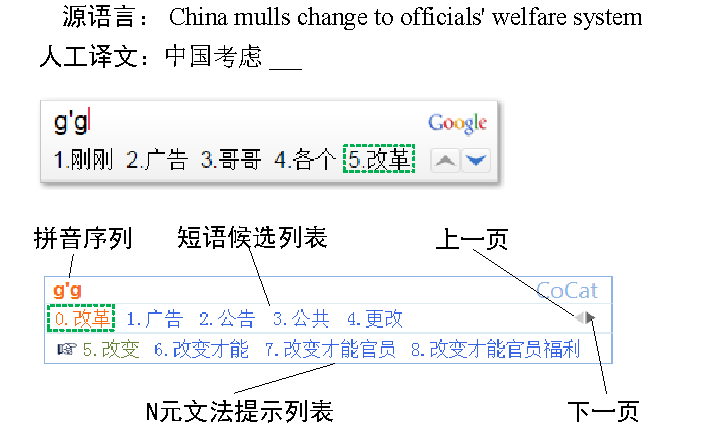
\includegraphics[width=0.8\textwidth]{Figure/Figure_3_2.pdf}
	\caption{谷歌拼音输入法与CoCat输入法的界面比较}
	\label{Fig_google_cocat_compare}
\end{figure}

\begin{figure}[tb]
	\centering
	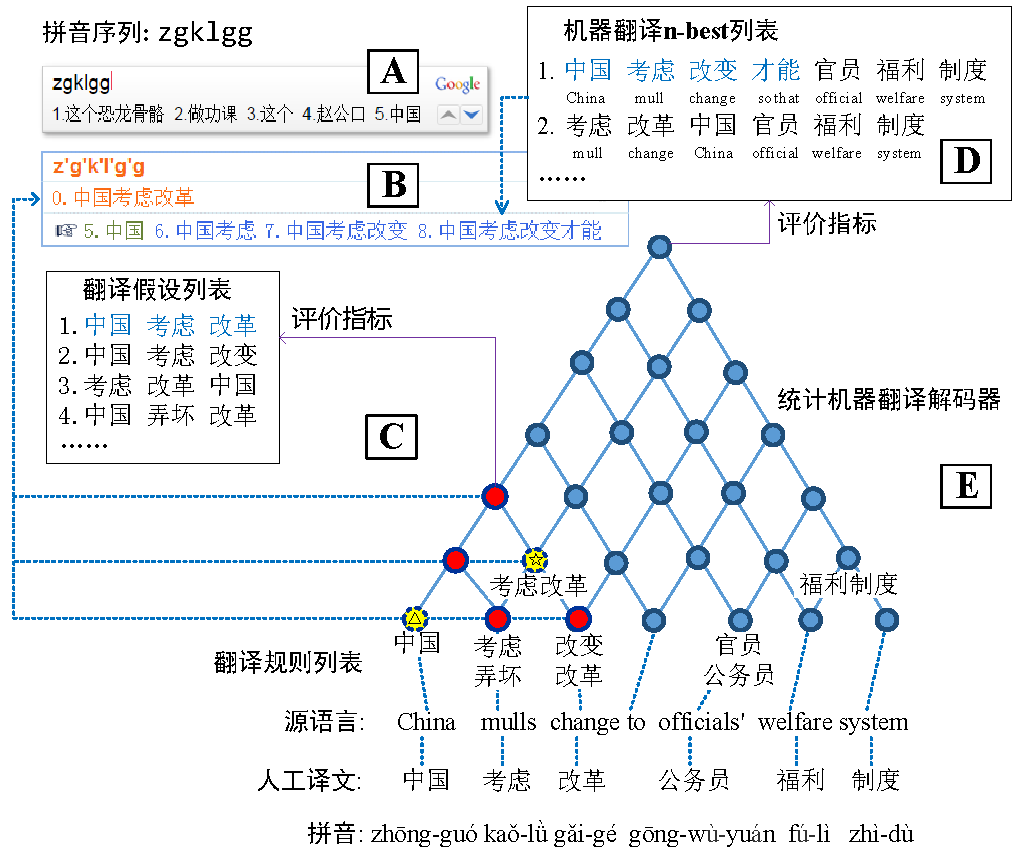
\includegraphics[width=0.98\textwidth]{Figure/Figure_3_3.pdf}
	\caption{CoCat输入法概览图}
	\label{Fig_cocat_overview}
\end{figure}

CoCat输入法与其它输入方法的主要区别在于,前者将统计机器翻译知识融合进人工翻译场景中的译文输入过程,而后者并不区别对待人工翻译场景。因此,CoCat包含两个面向计算机辅助翻译场景的新模型:输入法短语生成模型和N元文法提示模型。CoCat输入法概览图如图\ref{Fig_cocat_overview}所求。相对于传统输入法,图\ref{Fig_google_cocat_compare}和图\ref{Fig_cocat_overview}显示了CoCat输入法三方面的优势:

(1)利用从机器翻译系统抽取出的额外特征,输入法短语生成模型能根据当前上下文对目标短语进行重排序。如图\ref{Fig_google_cocat_compare}所示,输入拼音序列“gg”时,正确的输入法短语候选“改革”被CoCat排在第一,但是谷歌拼音输入法在相同情景下未能达到一样的效果。

(2)在统计机器翻译知识的帮助下,输入法短语生成模型还能为当前源语言句子生成新的输入法短语候选。如图\ref{Fig_cocat_overview}所示,输入拼音序列“zgklgg”时,谷歌拼音给出的输入结果与用户期待的结果相去甚远,但CoCat输入法利用翻译规则和翻译假设等翻译知识顺利得到正确的输入法短语候选“中国考虑改革”。

(3)N元文法提示模型根据已输入部分生成一系列N元文法提示。如图\ref{Fig_cocat_overview}所示,序号为5-8的四个短语即为N元文法提示模型的预测结果:“中国”、“中国考虑”、“中国考虑改变”和“中国考虑改变才能”。显然,“中国考虑”为正确结果。

\subsection{输入法短语生成模型}

我们的假设是,使用拼音输入法时,击键数越少,则打字速度越快,继而能留更多的时间让译员思考,最终在提升翻译效率的同时也提高翻译质量。因此,我们的目标是减少人工翻译过程中的按键数。如图\ref{Fig_cocat_overview}所示,在翻译示例中的源语言句子时,我们输入最短拼音串“zgklgg”,如果正确的结果“中国考虑改革”被排在第一位,我们就可以又好又快地完成翻译任务。而目前的谷歌拼音输入法、搜狗输入法等通用输入法并不能有效地感知人工翻译的上下文信息。幸运地是,在辅助翻译场景中,统计机器翻译系统中有输入法感知上下文所需要的相关信息。因此,为了达到这个目标,我们将机器翻译的相关特征引入公式\ref{input_method_linear}所示的CoCat输入法对数线性模型。在本章中,我们从统计机器翻译中抽取出六个特征:

(1)输入法短语候选中有多大比例的词在机器翻译n-best列表中;

(2)输入法短语候选是否包含在机器翻译n-best列表中的二值特征;

(3)输入法短语候选中有多大比例的词在翻译假设中;

(4)输入法短语候选是否在翻译假设中的二值特征;

(5)输入法短语候选中有多大比例的词在翻译规则中;

(6)输入法短语候选是否在翻译规则中。

我们使用CYK算法进行输入法解码[\cite{Kasami:1965,Younger:1967}],同时利用柱搜索(Beam-search)算法进行加速。

为了完成示例中的翻译任务,我们的按键序列如图\ref{Fig_cocat_enable_disable_prediction}(a)所示。之所以由拼音序列“zgklgg”能得到正确的结果“中国考虑改革”,是因为子串之一“中国”被包含在机器翻译翻译规则中(图\ref{Fig_cocat_overview}中的△),而另一子串“考虑改革”恰好在机器翻译解码器生成的翻译假设中(图\ref{Fig_cocat_overview}中的☆)。这样,“中国考虑改革”将在剪枝和重排序过程中得到比较高的分数。

\subsection{N元文法提示模型}

为了进一步减少翻译过程中的按键数,受拼音输入法的“词语联想”功能启发,我们提出了N元文法提示模型。

所谓N元文法提示是指:第一个提示短语为一元文法,只包含一个词;第二个提示短语为二元文法,包含两个词,且第一个提示短语是第二个提示短语的前缀;以此类推,第N-1个提示短语的所有词是第N个提示短语的前缀,第N个提示短语为N元文法包含N个词。N为正整数,默认值为4。

我们利用机器翻译结果的n-best列表,结合用户已录入部分进行最长后缀匹配而生成N元文法提示。假设机器翻译n-best列表为$O=\{O_i | 0 < i \le |O|\}$,第$i$个机器翻译候选$o_i=o_{i1}o_{i2} \ldots o_{i|o_i|}$。其中,$|O|$表示n-best列表长度,$|o_i|$表示机器翻译候选$o_i$的词数,$o_{ij}$表示机器翻译候选$o_i$的第$j$个词。令人工翻译译文为$t_1^m=t_1t_2 \ldots t_m$,则生成N元文法提示的步骤如下:

(1)当译员尚未输入目标译文时,已输入部分为空,利用最佳机器翻译候选的前N个词,生成初始N元文法提示列表为$\{p_l | p_l=o_{11} \ldots o_{1l} (1 \le l \le N)\}$;

(2)译员可以直接选择一个提示短语以快速输入,也可以选择忽略;

(3)当译员输入译文的第$m'$个词$t_{m'}$之后,已录入部分为$t_1^{m'}=t_1 t_2 \ldots t_{m'}$,我们从$O$中尝试找到与$t_1^{m'}$最长后缀匹配的机器翻译候选$o_i$;

(4)如果成功找到$o_i $,则继续利用最长后缀匹配算法找到$k$使其满足$o_{ik}=t_{m'}$,则更新N元文法提示列表为$P=\{p_l |p_l=o_{i(k+1)}  o_{i(k+2)} \ldots o_{i(k+l)} (1 \le l \le N)\}$;如果词$t_{m'}$未出现在机器翻译n-best列表中的候选译文,则N元文法提示列表为空;

(5)回到步骤(2),直到译员完成翻译。

\begin{figure}[hbp]
	\centering
	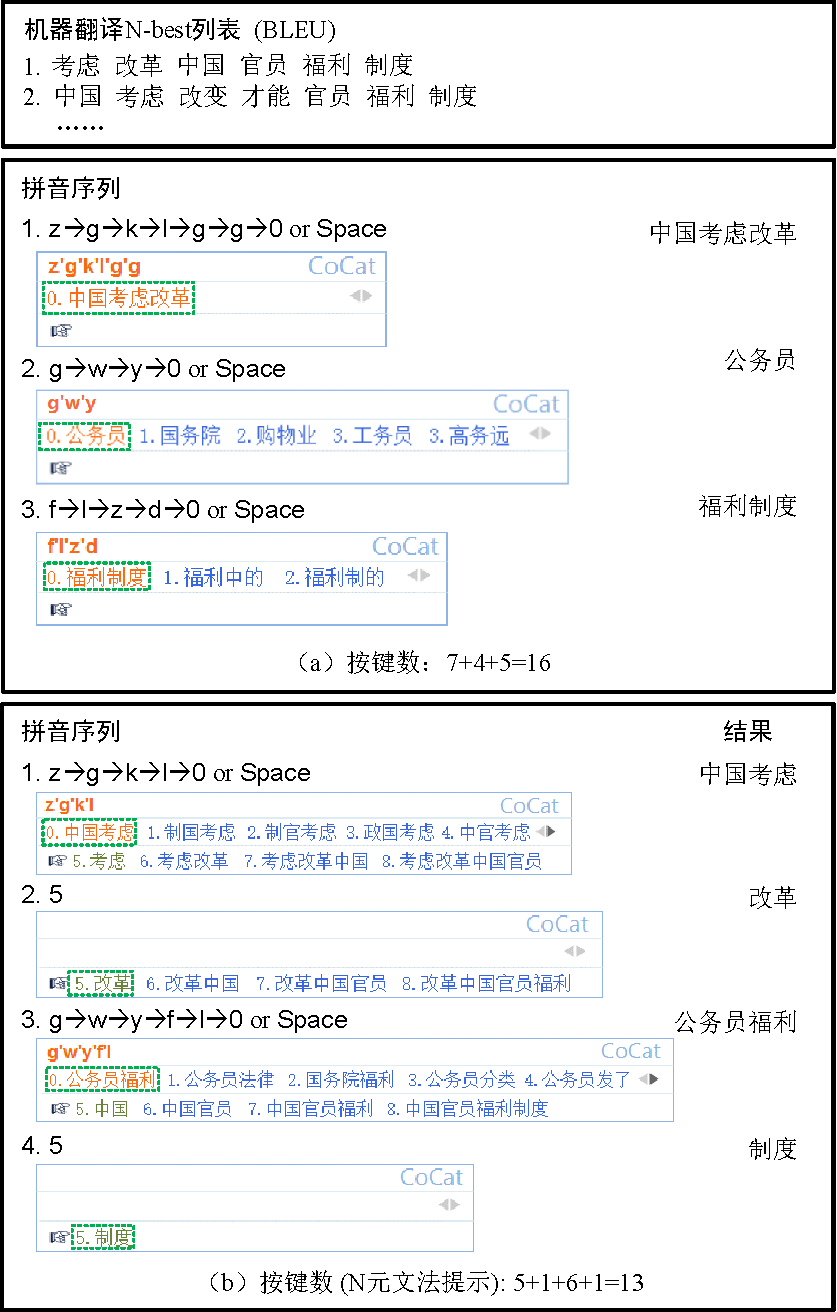
\includegraphics[width=0.98\textwidth]{Figure/Figure_3_4.pdf}
	\caption{禁用/启用N元文法提示的输入法按键序列比较}
	\label{Fig_cocat_enable_disable_prediction}
\end{figure}

如果我们启用N元文法提示模型,则完成示例中的翻译任务时的按键序列如图\ref{Fig_cocat_enable_disable_prediction}((b)所示。在步骤2中通过数字键“5”直接选择正确的N元文法提示“改革”,以及在步骤4中直接选择正确的翻译提示“制度”,我们可以节省的按键数为:

$$\frac{16-13}{16} \times 100\% = 18.75\%$$

这样,即便机器翻译结果质量不高,CoCat输入法也能改善人机交互体验,从而帮助译员提高生产效率。

综上所述,CoCat输入法通过两方面提升人工翻译效率:(1)译员不需要阅读并评估机器翻译自动译文,输入方法自动地将机器翻译系统中的翻译知识融合进输入过程,结合当前上下文信息,生成更合适的输入法短语候选,并对输入法短语候选进行重排序;(2)根据机器翻译n-best列表提供N元文法提示,使译员更方便地选择统计翻译的高质量片断。

\section{面向输入方法的译文自动评价指标}

在图\ref{Fig_cocat_overview}中,统计机器翻译解码器利用如下对数线性模型对翻译规则、翻译假设和n-best翻译候选进行排序:

\begin{equation}
\log p(t|s)= \sum_{m=1}^{M}\lambda'_m f_m(t,s)
\end{equation}

其中$s$和$t$分别表示源语言句子和翻译候选。通常而言,该对数线性模型的特征$ \{f(t,s)\}$包括翻译模型概率、目标语言模型概率、调序模型概率等。参数调节(parameter tuning)的任务就是学习特征$f_m(t,s)$的权重$\lambda'_m$,通常称之为最小错误率训练(minimum error rate training,MERT)。

\begin{figure}[!btp]
	\centering
	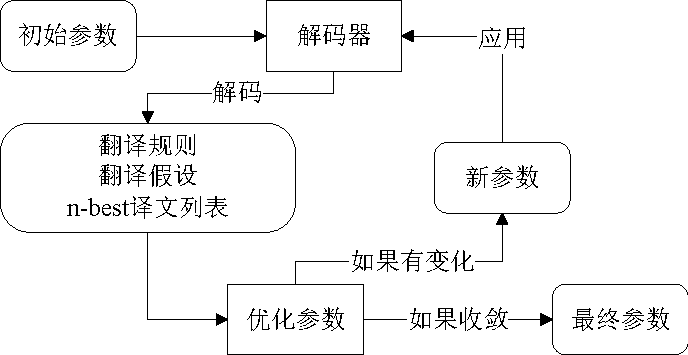
\includegraphics[width=0.8\textwidth]{Figure/Figure_3_5.pdf}
	\caption{迭代式的最小错误率训练}
	\label{Fig_mert}
\end{figure}

参数调节过程是利用具体的译文自动评价指标实现的。常用的译文自动评价指标包括BLEU和TER。如图\ref{Fig_cocat_enable_disable_prediction}中所示统计机器翻译系统即为用BLEU作为最小错误率训练的评价指标。

用于参数调节的训练集称为开发集。在参数调节的开始状态,一个可能包含一千个双语平行句对的开发集,利用初始设定的参数值获得n-best译文列表。我们需要对所有可能的参数设置在n-best译文列表上的效果进行打分。每种译文都可能成为“最佳”译文,通常情况下我们使用BLEU或者TER来衡量自动译文的翻译误差。最终搜索到与采用的评价指标对应的最优参数即为对数线性模型中$\{\lambda'_m\}$的值。

在统计机器翻译解码过程中,$\{\lambda'_m\}$的值会直接影响到翻译规则、翻译假设和n-best译文列表中的元素及其排序,因为得分过低的元素会被剪枝。而CoCat输入法的性能与翻译规则、翻译假设和n-best译文列表中的元素及其排序直接相关。可见,译文自动评价指标会影响CoCat输入法的性能。

由此可知,如果我们为CoCat输入法精心设计在统计机器翻译系统的最小错误率训练过程中所使用的译文自动评价指标,或者适当调整参数调节过程中的一些细节,则有可能进一步减少译员翻译过程中的按键数。
但是目前已有的译文自动评价指标并不适合我们提出的CoCat输入法的。

为了达到我们的目的,我们提出了专门针对CoCat输入法的译文自动评价指标MinKSR。MinKSR的评价对象由n-best译文即句子级别扩展到CoCat输入法依赖的深层次翻译知识:翻译规则、翻译假设和n-best译文。MinKSR衡量的是当前参数产生的翻译知识能为CoCat节省多少按键数。另外,单就句子级别而言,MinKSR直接奖励最长匹配片断。图\ref{Fig_mert}表示利用MinKSR进行的最小错误率训练。解码器产生用于优化参数的深层次翻译知识,如翻译规则、翻译假设和n-best译文列表。然后根据产生的深层次翻译知识评估按键数,并更新参数。利用新的参数运行解码器,不断循环这个过程,直到按键数不再减少。

\subsection{MinKSR}

MinKSR的目的是衡量与CoCat输入法融合的机器翻译系统最少能帮助译员节省多少按键数。核心思想是更长的匹配片断消耗更少的按键数。自动计算一段文本的实际按键数不是容易的事,因此我们用“经验按键数”代替实际按键数。所谓经验按键数,指实际按键数的一个可能下限值,即除了极少数特例,输入同一段文本的实际按键数都不会低于这个值。

MinKSR包含三个重要的统计量:

(1) $mk_{norm}(t_1^m)$:逐字独立录入参考译文 的理论最少按键数。

(2) $ek(Q, t_1^m)$:结合待评价机器翻译结果$ t_1^m=t_1t_2 \ldots t_m$录入参考译文的最少按键数。其中,机器翻译结果$Q=\{L,H,C\}$为包括机器翻译系统的翻译规则集合$L$、翻译假设集合$H$和n-best译文集合$C$的三元组。

(3) $pk(t_1^m)$:结合理想机器翻译结果录入参考译文$t_1^m$的理论最少按键数。理想机器翻译知识可简化为最终的机器翻译自动译文与参考译文一致。

借助上述三个统计量,我们便可以结合参考译文计算待评价机器翻译结果$Q$ \linebreak
的MinKSR值。令源语言句子为$s_1^j=s_1s_2 \ldots s_j$,翻译规则集合$L=\{l_1^{Z_1}\}$,翻译假设集合$H=\{h_1^{Z_2}\} $,n-best译文集合$C=\{c_1^{Z_3}\}$。其中,$Z_1$表示统计机器翻译解码器翻译规则表最大长度限制,$Z_2$表示解码过程中柱搜索时单个短语的翻译假设列表最大长度限制,$Z_3$表示n-best列表最大长度限制。给定待评价机器翻译结果$Q$和参考译译文$ t_1^m=t_1t_2 \ldots t_m$,则$Q$的MinKSR的分值$r$可以根据下列公式计算得到:

\begin{equation}
\label{minksr_raw}
r(Q,t_1^m)=\frac{mk_{norm}(t_1^m)-ek(Q,t_1^m)}{mk_{norm}(t_1^m)-pk(t_1^m)}
\end{equation}

如果机器翻译结果$Q$只有n-best译文,则MinKSR的行为与BLEU类似。如果有多个参考译文,我们就选择使$ek(Q, t_1^m)$值最小的那个参考译文计算。

为了使公式3.3独立于具体语言,我们还需要引入下列经验参数:

\begin{itemize}
	\item $sn$:句子中词之间的分隔符个数:对于汉语,$sn=0$;但对于英文,因为用一个空格隔开相邻的两个单词,因此$sn=1$。
	
	\item $kc$:从输入法界面上选择一个输入法短语候选或者N元文法提示的按键数。一般而言,$kc=1$。
	
	\item $rk$输入一个词的按键数与字符数的比值。由3.2节讨论可知,输入一个汉字的平均按键数为2.1,因此我们取$rk=2$以保证公式\ref{minksr_raw}的结果是机器翻译知识最少能帮助译员节省的按键数。
\end{itemize}

为了公式3.3,我们首先要计算$mk_{norm}(t_1^m)$、$ek(Q, t_1^m)$、$pk(t_1^m)$等三个统计量的值:

(1)逐字独立录入参考译文的理论最少按键数:
\begin{equation}
mk_{norm}(t_1^m) = \sum_{i=0}^m (mkw_{norm} (t_i)+sn+kc)-sn
\end{equation}
其中,$mkw_{norm} (t_i)$表示输入词$t_i$所需要的按键数:
\begin{equation}
mkw_{norm} (t_i)=len(t_i) \times rk
\end{equation}
其中,$len(t_i)$表示词 的字符数。

(2)结合待评价机器翻译结果录入参考译文的最少按键数:
\begin{equation}
ek (Q,t_1^m) =\min_{cp_1^q \in CP(t_1^m)} \left\{ \sum_{i=1}^q {(ek(Q,cp_i)+sn)-sn} \right\}
\end{equation}
其中,$CP(t_1^m)$表示参考译文所有不同的划分,每个划分$cp$表示译员对参考译文的一种短语切分方式;$q$表示对应划分的短语数目,短语是译员使用输入法时一个连续拼音串对应一个短语;$ek(Q,cp_i)$表示结合待评价机器翻译结果$Q$输入短语$cp_i$的最小按键数。划分的最小元素是词。令$P$为输入短语$cp_i$时的N元文法提示列表,则$ek(Q,cp_i)$的值可以由下述公式计算得出:
\begin{equation}
\label{minksr_ek}
ek(Q,cp_i) = \left \{ 
\begin{array}{ll}
kc & cp_i \in P \\
len(t_i)+kc & cp_i \notin P,cp_i \in Q \\
mkw_{norm}(cp_i)+kc & cp_i\notin P,cp_i \notin Q \\
\end{array}
\right. 
\end{equation}

公式\ref{minksr_ek}是MinKSR的核心,其基本思想是尽可能直接选择正确的N元文法提示完成输入,此时一个按键就能输入短语$cp_i$。如果没有正确的N元文法提示,则尽量由待评价机器翻译结果 中的词组成短语,此时的理想情况是通过每个字的拼音首字母就能输入该短语。如果N元文法提示和待评价机器翻译结果同时命中失败,则退回到普通输入法。

\begin{figure}[!hbt]
	\centering
	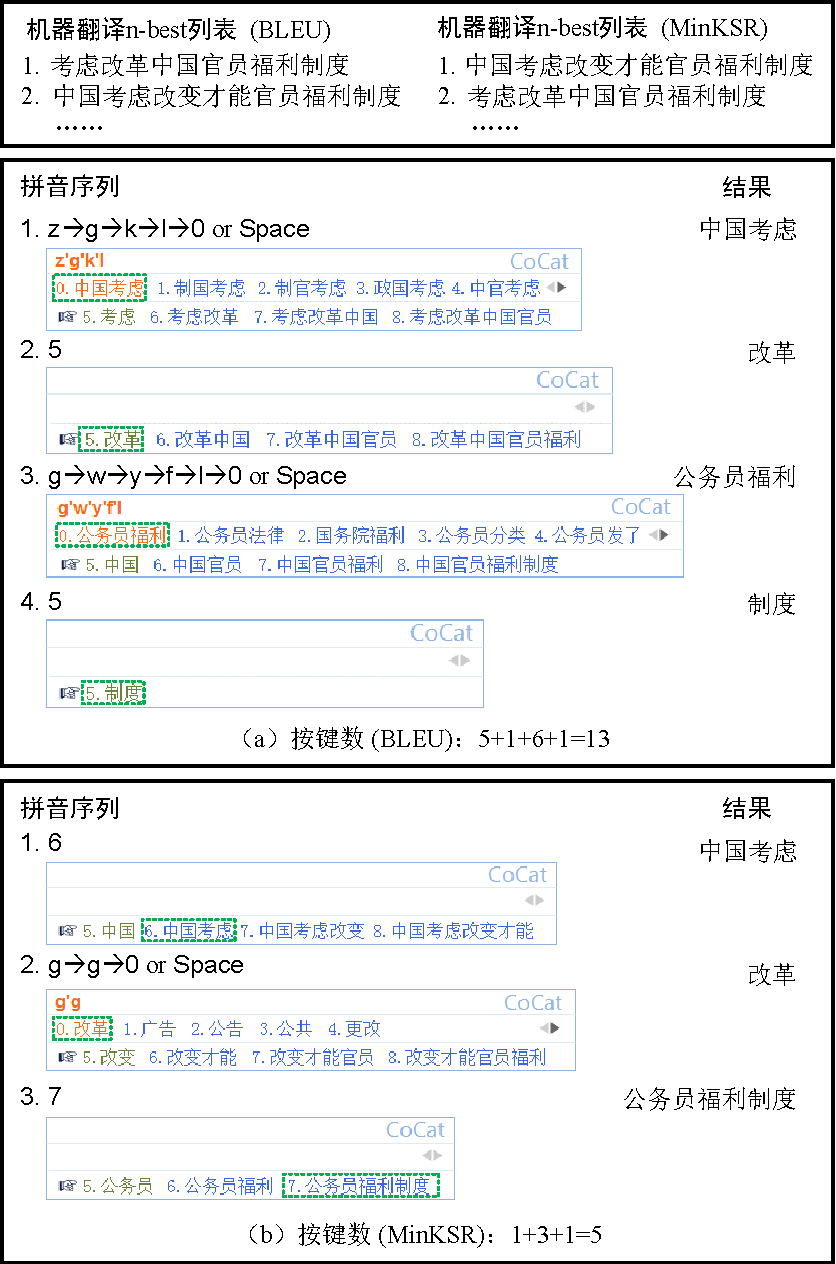
\includegraphics[width=0.98\textwidth]{Figure/Figure_3_6.pdf}
	\caption{基于BLEU/MinKSR的输入法按键序列比较}
	\label{Fig_keystroke_bleu_minksr}
\end{figure}

(3)结合理想机器翻译结果录入参考译文的理论最少按键数:
\begin{equation}\label{minksr_pk}
pk (t_1^m) = \left \{ 
	\begin{array}{ll}
		\frac{m}{N} \times (kc+sn)-sn & m\;mod\; N=0 \\
		\lfloor \frac{m}{N} \rfloor \times (kc+sn)+kc & m\;mod\;N \not = 0 \\
	\end{array}
	\right. 
\end{equation}
其中,$N$为N元文法提示的个数,默认值为4。

公式\ref{minksr_pk}表示当机器翻译结果完全符合要求时,译员可以仅通过N元文法提示输入参考译文。

综上所述,我们可以通过公式\ref{minksr_raw}计算单个源语言句子对应的机器翻译知识的MinKSR值。而语料级的MinKSR值可由下列公式计算得出:
\begin{equation}
\label{minksr_multi_ref}
r = \frac{\sum_{t\in T}mk_{norm}(t)-\sum_{t\in T,Q\in \{Q\}}ek(Q,t)}
{\sum_{t\in T}mk_{norm}(t)-\sum_{t\in T}pk(t)}
\end{equation}
其中,$T$表示所有源语言句子对应的参考译文集合。

\subsection{译文长度惩罚因子}

公式\ref{minksr_raw}和\ref{minksr_multi_ref}考虑了n-best译文中词和词的顺序,但没有考虑目标译文长度。令$c$为n-best译文列表中自动译文的平均长度,$t$为参考译文的平均长度。受BLEU启发,MinKSR的译文长度惩罚因子BP为:
\begin{equation}
BP= \left \{ 
\begin{array}{ll}
1 \ & if \ c \le t \\
e^{1-\frac{c}{t}} \ & if \ c>t \\
\end{array}
\right.
\end{equation}
因此,最终的MinKSR得分计算公式为:
\begin{equation}
MinKSR=BP \times r
\end{equation}

MinKSR值的范围为[0,1],得分越高,机器翻译结果越好,意味着可以节省人工翻译过程中更多的按键数。完美机器翻译结果的MinKSR分值为1。

我们以图\ref{Fig_keystroke_bleu_minksr}为例说明MinKSR在辅助翻译场景中是如何工作的。图\ref{Fig_keystroke_bleu_minksr}(a)和图\ref{Fig_keystroke_bleu_minksr}(b)中CoCat输入法依赖的分别是用BLEU和MinKSR进行最小错误率训练之后的统计机器翻译系统。为简洁起见,我们仅列出了n-best译文中的前两句译文候选,省略了统计机器翻译解码器的深层次信息和完整的n-best译文列表。可见,前两句译文候选被MinKSR调换了位置,造成的结果是按键数从13减少到5。图\ref{Fig_keystroke_bleu_minksr}(b)中的关键步骤是1和3:在步骤1中,CoCat借助n-best译文直接生成了完全正确的N元文法提示“中国考虑”;在步骤3中,CoCat如法炮制,生成了正确的翻译提示“公务员福利制度”。由此可以说明n-best译文等深层次信息对CoCat输入法是非常重要的。

\section{相关工作}

CoCat输入法的目的是通过充分利用机器翻译知识来提高专业译员的翻译效率。其核心思想是以一种人机友好且有效的方式提高输入速度。如下有两种类型的相关工作也专注这个问题。

首先是Koehn等人[\cite{Koehn:2009a,Koehn:2014}]与Green[\cite{Green:2014}]等人开发的交互式机器翻译系统。前者是名叫“Caitra”的翻译工具,旨在为译员完成目标译文,实时提供词和短语的译文建议。后者为人工翻译设计了新的计算机辅助翻译界面,同时也根据用户已录入的部分提供实时的译文建议。这两个系统都要求译员必须从左至右完成翻译,并没有脱离交互式机器翻译的限制,同时需要绑定从左至右进行解码的机器系统。而我们提出的CoCat输入法并没有这些限制,不与任何特定类型的机器翻译解码器进行约束和绑定,而仅是将机器翻译的翻译知识以特征的形式加入到输入法的对数线性模型中。同时,CoCat输入法并不要求译员注意到机器翻译系统的存在,还可以与现有的译后编辑和交互式机器翻译方式配合使用。因此,CoCat输入法在提高人工翻译效率的同时提供了更好的人机交互体验。

其次是厦门大学史晓东教授团队也在面向计算机辅助翻译场景的中文输入方法方面有重要尝试[\cite{lidong:2006,LiDong:2012,fang:2013}]。在他们的方法中,输入方法仅用了机器翻译模型针对输入法短语候选输出的分数和模糊词对齐信息。因此,他们的方法有两个不足:(1)机器翻译模型动态输出的分数难以计算,且很难与输入法其它特征的值进行融合;(2)输入法短语候选与源语言句子的模糊词对齐中包含很多噪声,尤其是当自动译文与人工译文的差异比较大的情况下,模糊词对齐信息对输入法的帮助极其有限。我们提出的面向计算机辅助翻译的输入法将翻译规则、翻译假设列表和翻译结果候选列表等统计机器翻译深层次知识融合进输入法的对数线性模型,从而生成更准确的输入候选列表和短语提示列表。在人工译文与自动译文差距较大的情况下,通过巧妙地特征设计,CoCat输入法自动退化为普通输入法,不会受到机器翻译的干扰。另外,我们还设计了N元文法提示模型以进一步提高人工翻译效率。

\section{实验}

本节将探讨CoCat输入法和MinKSR评价指标在提高人工翻译效率方面的性能。输入法方面,与CoCat进行比较的是谷歌拼音输入法和译后编辑;评价指标方面,与MinKSR进行比较的是BLEU和TER。我们将从三方面考查人工翻译效率,分别是:翻译时间、按键数和翻译质量。

\subsection{实验设置}

本章中所有实验都是基于元辅翻译平台(CoTrans)。该平台集成计算机辅助翻译系统和基于短语翻译模型的统计机器翻译系统。该平台支持多种语言对,就本章而言,我们的实验仅针对英到汉的人工翻译任务。集成的机器翻译系统的训练集为约1千万的新闻平行句对,开发集包含1000平行句对,最小错误率训练工具和评价指标分别为ZMERT和TER。开发集的源文即英语句子选自截止到2014年3月的China Daily网站时政新闻栏目,再由专业译员翻译成中文。统计显著性检验使用重采样方法。CoTrans翻译平台会记录译员的每次按键和鼠标操作,最后生成用户交互日志以方便我们分析所有细节,包括用户的翻译时间、按键数和翻译质量。

下面,我们将介绍参与实验的专业译员和实验数据。

\textbf{(1)专业译员}

参考计算机辅助翻译相关实验惯例,我们邀请了12位母语为中文的专业译员参与该实验。这12名专业译员包括高校翻译专业教师、全职译员、自由译员和高校研究生,平均翻译水平能代表当前翻译市场的主流程度。我们将所有译员平均分成四组(A/B/C/D),且每位译员翻译的句子与其他译员的是相同的。

\textbf{(2)人工翻译实验数据}

\begin{table}[htbp]
	\centering	
	\begin{tabular}{|c|c|c|c|}
		\hline
		\multicolumn{4}{|c|}{英语-汉语}                            \\ \hline
		\multicolumn{1}{|l|}{译员数\#} & \multicolumn{3}{c|}{12}  \\ \hline
		\multicolumn{1}{|l|}{男/女}   & \multicolumn{3}{c|}{6/6} \\ \hline
		\multicolumn{4}{|c|}{测试数据(英文单词数)}                      \\ \hline
		\multicolumn{1}{|l|}{}      & BLEU   & TER   & MinKSR  \\ \hline
		总数                          & 3918   & 3849  & 4102    \\ \hline
		$M_1$                        & 990    & 1031  & 1058    \\ \hline
		$M_2$                        & 983    & 966   & 1012    \\ \hline
		$M_3$                        & 969    & 980   & 1025    \\ \hline
		$M_4$                        & 976    & 882   & 1007    \\ \hline
	\end{tabular}
	\caption{测试数据}
	\label{Table_minksr_test_set}
\end{table}

\begin{table}[htbp]
	\centering
	\begin{tabular}{|c|c|c|c|c|}
		\hline
		& A  & B  & C  & D  \\ \hline
		Google    & $M_1$ & $M_4$ & $M_3$ & $M_2$ \\ \hline
		CoCat     & $M_2$ & $M_1$ & $M_4$ & $M_3$ \\ \hline
		PE+Google & $M_3$ & $M_2$ & $M_1$ & $M_4$ \\ \hline
		PE+CoCat  & $M_4$ & $M_3$ & $M_2$ & $M_1$ \\ \hline
	\end{tabular}
	\caption{翻译任务分配}
	\label{Table_minksr_task_assignment}
\end{table}

我们从截止到2014年12月的China Daily网站时政新闻栏目中选择出480句英文句子作为测试集$S=\{ s_i |i=1,2, \ldots ,480 \}$。该测试集包含11869个英文单词,每个句子的长度为23到26个英文词。

我们让每个译员用四种不同的辅助方式完成翻译任务:(1)谷歌拼音(``Google'');(2)CoCat输入法(``CoCat''); (3)译后编辑+谷歌拼音(``PE+Google'');(4)译文编辑+\linebreak
CoCat输入法(``PE+CoCat'')。需要注意的是,一个译员不能用不同的辅助方式翻译同样的句子,因为无论用什么辅助方式,第二次翻译相同句子时的速度几乎肯定比第一次翻译时快。四种辅助方式与三种评价指标共12种组合方式。所以,我们将测试集随机等分成4组共12份,每组3份,每份40句。一种辅助方式对应一组测试数据,这种辅助方式依赖的每种译文自动评价指标对应一份测试数据。测试数据的详细说明见表\ref{Table_minksr_test_set},四组测试数据分别标号为$M_1/M_2/M_3/M_4$。例如,$M_1$组中包括3份测试句子,用于BLEU的一份40句共有990个英文单词,用于TER的另外一份40句共有1031个英文单词,剩下的用于MinKSR的一份40句包含1058个英文单词。

翻译任务分配方式如表\ref{Table_minksr_task_assignment}所示。以BLEU为例,A组译员一共翻译160个不同的英文句子:先用谷歌拼音翻译第一份40句,后用CoCat翻译第二份40句,再用谷歌拼音结合译后编辑完成第三份40句翻译,最后用CoCat结合译后编辑翻译完成第四份40句。同组内部3人的任务序列一致。待翻译的英文句子长度被控制为23~26个词,480句共11869个英文词,连续翻译时间两天共超过20小时。作为参考,专业译员平均每天仅能高质量完成不超过5000词的翻译任务,因此本实验已达到压力测试要求。

需要说明的是,在人工翻译过程中,有很多因素会影响到最终的实验结果,如不同句子的难易程度、不同译员的翻译能力及连续长时间翻译的容忍程度。为了尽可能降低这些不相关因素的影响,我们根据表\ref{Table_minksr_task_assignment}分配翻译任务。这种分配方式基于以下假设:四组共12份英文句子的难度差异可以忽略;同一位参与的译员在不同时间的辛苦程度和翻译效率的差异均可以忽略。

\subsection{数据清洗}

为了排除如搜索查证和休息等与翻译不相关的因素,我们对交互日志数据作了如下处理:

(1)从时间线上删除所有与辅助方式不相关的交互,如在术语词典中查词、用搜索引擎在线查证;

(2)计算翻译时间时排除所有超过10秒钟的间隔;

(3)计算翻译质量得分时,对每一句话,从12名译员的翻译结果中选择最好的4个目标译文作为标准译文,然后根据标准译文分别计算其它未选中译文的BLEU分值。标准译文得分为1。


\subsection{数据处理}

我们通过翻译时间、按键数和翻译质量来分析人工翻译效率。为了增强数据的可靠性,我们对数据结果的处理采用多次重复实验然后求平均的思路。以“翻译时间”为例说明数据处理过程。

根据表3.2中的翻译任务分配,测试BLEU对翻译效率的影响时,$M_1$组中的源语言句子$s_i$会被A组译员用谷歌拼音输入法翻译3次。我们将这3次翻译的时间求平均而得到句子$s_i$用谷歌拼音输入法的翻译时间$time_{s_i}^{Google}$。然后,我们用下列公式计算$M_1$组译文用谷歌拼音输入法的翻译时间:
\begin{equation}
time_{M_1}^{Google} = \frac{\sum_{s_i \in M_j} time_{s_i}^{Google}}{|M_1|}
\end{equation}
B、C、D组译员分别用谷歌拼音输入法翻译$M_4$、$M_3$、$M_2$组译文,然后用同样的方式得到各组译文用谷歌拼音输入法的翻译时间。同理,我们用下列公式针对所有句子经谷歌拼音输入法的翻译时间求平均,从而得到最终的谷歌拼音输入法翻译时间:
\begin{equation}
time^{Google} = \frac{\sum_{i=1}^{160} time_{s_i}^{Google}}{160}
\end{equation}
用相同的处理方式可以得到按键数和翻译质量的结果。

\subsection{结果分析}

\textbf{(1)输入方法实验}

\begin{table}[htbp]
	\centering
	\begin{threeparttable}
		\begin{tabular}{*{7}{|c}|}
			\hline
			& 辅助方式 & A & B & C & D & 平均 \\
			\hline
			\multirow{6}{*}{\rotatebox{90}{翻译时间}}  & Google & 114.68 & 110.67 &  80.39 & 100.30 & 102.38 \\
			\cline{2-7}
			&  \multirow{2}{*}{CoCat} &  89.61** &  98.05** &  68.05** &  71.56** &  \textbf{84.03}** \\
			&                         & (21.86\%$\downarrow$) & (11.40\%$\downarrow$) & (15.35\%$\downarrow$) & (28.65\%$\downarrow$) & (\textbf{17.89\%}$\downarrow$)\\
			\cline{2-7}
			& PE+Google &  64.70 &  52.93 &  83.25 &  71.78 &  66.59 \\
			\cline{2-7}
			&  \multirow{2}{*}{PE+CoCat} &  52.03** &  48.34** &  65.43** &  66.90** &  \textbf{56.63}** \\
			&                            &  (19.58\%$\downarrow$) & (8.68\%$\downarrow$) & (21.41\%$\downarrow$) & (6.80\%$\downarrow$) & (\textbf{14.97\%}$\downarrow$)\\
			\cline{1-7}
			\multirow{6}{*}{\rotatebox{90}{敲键数}}   &    Google & 209.83 & 236.78 & 168.65 & 184.30 & 204.26 \\
			\cline{2-7}
			&   \multirow{2}{*}{CoCat} & 138.41** & 168.13** &  93.94** & 124.33** & \textbf{134.85}** \\
			&                          & (34.04\%$\downarrow$) & (28.99\%$\downarrow$) & (44.30\%$\downarrow$) & (32.50\%$\downarrow$) & \textbf{(33.98\%}$\downarrow$)\\
			\cline{2-7}
			& PE+Google & 100.66 &  92.24 & 158.13 & 121.81 & 115.75 \\
			\cline{2-7}
			&  \multirow{2}{*}{PE+CoCat} &  59.36** &  63.44** &  80.77** &  82.11** &  \textbf{69.87}** \\
			&                            &  (41.03\%$\downarrow$) & (31.22\%$\downarrow$) & (48.92\%$\downarrow$) & (32.60\%$\downarrow$) & (\textbf{39.64\%}$\downarrow$)\\
			\cline{1-7}
			\multirow{6}{*}{\rotatebox{90}{翻译质量}} &    Google &  68.17 &  72.25 &  75.96 &  71.57 &  72.12 \\
			\cline{2-7}
			&     \multirow{2}{*}{CoCat} &  73.72** &  78.15** &  83.63** &  79.64** &  \textbf{78.73}** \\
			&                            &  (8.14\%$\uparrow$) & (8.17\%$\uparrow$) &  (10.10\%$\uparrow$) & (11.27\%$\uparrow$) & (\textbf{9.17\%}$\uparrow$)\\
			\cline{2-7}
			& PE+Google &  78.49 &  80.74 &  77.02 &  77.72 &  78.79 \\
			\cline{2-7}
			&  \multirow{2}{*}{PE+CoCat} &  81.53** &  85.32** &  82.43** &  72.76 &  \textbf{81.98}** \\
			&                            &  (3.04\%$\uparrow$) & (4.58\%$\uparrow$) &  (7.03\%$\uparrow$) & (4.96\%$\downarrow$) & (\textbf{3.19\%}$\uparrow$)\\
			\cline{1-7}
			\hline	
		\end{tabular}
	\end{threeparttable}
	\caption{不同辅助方式之间翻译时间、按键数和翻译质量的比较}
	\label{Table_minksr_time_keystroke_quality}
\end{table}

不同辅助方式的翻译效率的详细统计数据如表\ref{Table_minksr_time_keystroke_quality}所示。括号中的数字表示当前行相比于上一行提高的百分比。如表\ref{Table_minksr_time_keystroke_quality}所示,由于人工实验中影响实验结果的因素比较多,不同组别的差异相对比较大。但就平均而言,我们可以发现,相对于仅用谷歌拼音输入法,无论是译后编辑还是CoCat输入法都能使人工翻译相对更快更好地完成翻译任务。同时,无论是否结合译后编辑,CoCat输入法的翻译效率和翻译质量都高于谷歌拼音输入法。

对于翻译时间和按键数而言,数值越低越好。相对于谷歌拼音输入法而言,表\ref{Table_minksr_time_keystroke_quality}中的粗体字表明CoCat输入法帮助译员减少超过14\%的翻译时间和超过33\%的按键数,且统计显著($p<0.01$)。例如同在译后编辑模式下,即第4行与第3行比较,CoCat输入法帮助译员减少了14.97\%的翻译时间;如果不借助译后编辑,即第2行与第1行比较,译员从空白开始翻译,则CoCat输入法相对于谷歌拼音输入法则更有优势。另外,第8行的粗体字表示在译后编辑模式下的按键数方面,相比于谷歌拼音输入法,CoCat输入法更有优势。

针对某个具体译员而言,如C组的一位女性译员,她翻译每句话的翻译时间和按键数记录分别如图\ref{Fig_translator_time}和图\ref{Fig_translator_keysroke}所示,也充分说明了CoCat输入法的优越性。

\begin{figure}[!htb]
	\centering
	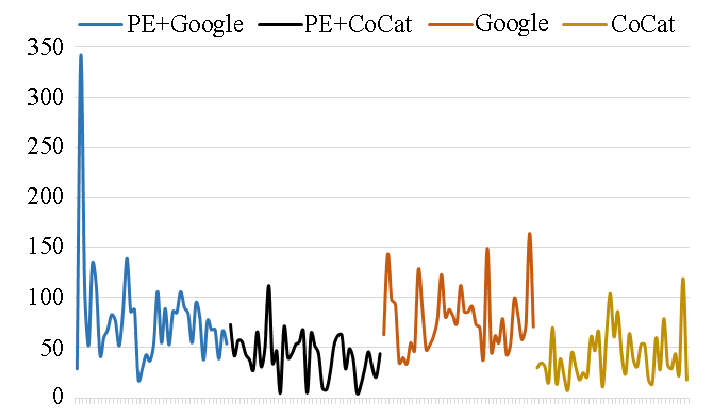
\includegraphics[width=0.85\textwidth]{Figure/Figure_3_7.pdf}
	\caption{某译员的翻译时间记录。纵坐标表示翻译时间(秒),横坐标表示句子ID}
	\label{Fig_translator_time}
\end{figure}

\begin{figure}[!htb]
	\centering
	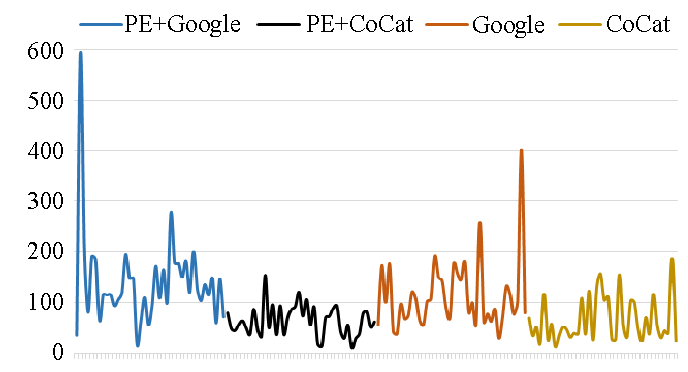
\includegraphics[width=0.85\textwidth]{Figure/Figure_3_8.pdf}
	\caption{某女性译员的翻译按键数记录。纵坐标表示按键数,横坐标表示句子ID}
	\label{Fig_translator_keysroke}
\end{figure}

\begin{figure}[!htb]
	\centering
	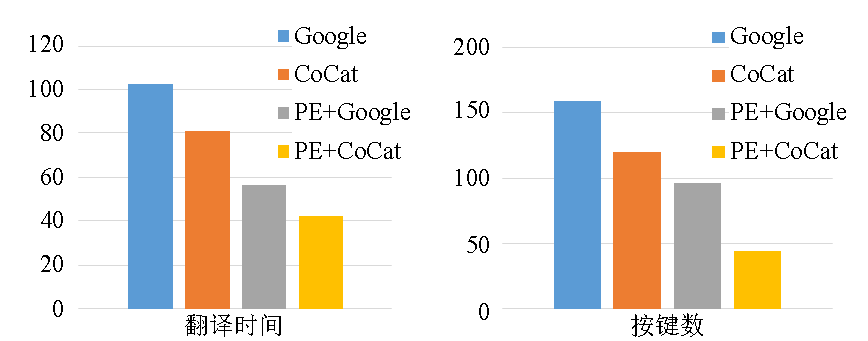
\includegraphics[width=0.85\textwidth]{Figure/Figure_3_9.pdf}
	\caption{具体句子的翻译时间和按键数比较}
	\label{Fig_sentence_keysroke}
\end{figure}

以一个具体的原文句子“CPC's discipline agency announced on Jan. 16 that Huo has been placed under investigation for suspected serious violation of party disciplines and laws”为例,CoCat输入法与谷歌拼音输入法在翻译时间和按键数的比较如图\ref{Fig_sentence_keysroke}所示。如果不用译后编辑模式,CoCat输入法可以节省约21\%的翻译时间和约24\%的按键数;如果启用译后编辑模式,CoCat输入法可以帮助译员节省约26\%的翻译时间和约53\%的按键数。

对于翻译质量而言,BLEU分值越高越好。表\ref{Table_minksr_time_keystroke_quality}中,第10行和第12行的粗体字表明CoCat输入法相对于谷歌输入法而言,可以提升超过3个BLEU值。第10行的粗体字表明,如果纯粹从空白开始翻译,CoCat输入法相对于谷歌输入法有更好的优势。第12行的粗体字表明CoCat输入法与译后编辑结合后能取得更好的翻译质量。

同时,表\ref{Table_minksr_time_keystroke_quality}表明了译后编辑总能提升翻译效率,这与已有文献的结论相吻合。另外,如果关注CoCat输入法与译后编辑模式下的谷歌拼音输入法,我们可以发现二者的翻译质量差别非常小。而在实际生产环境中,译员对直接更改机器翻译结果的意愿并不强烈。实际的译员反馈表明,借助CoCat输入法,虽然翻译时间和按键数比在译后编辑模式下的谷歌拼音输入法相对多一些,但CoCat输入法并不强迫译员阅读和分析机器翻译结果,从而实际上提高了人工翻译效率,所以译员实际更倾向于使用CoCat输入法。

综上所述,通过实验数据我们可以作如下结论:CoCat输入法确实改善了机器翻译的人机交互体验,在不增加译员负担的情况下,提高了人工翻译生产效率。

\textbf{(2)译文自动评价指标实验}

为了继续改进CoCat输入法的翻译效率,接下来我们比较MinKSR相对于BLEU\linebreak
和TER在输入法场景下的性能差异。译文自动评价指标实验包括比较测试、相关性测试和人工测试。

\textbf{(2.1)比较测试}

\begin{table}[!b]
		\begin{threeparttable}
			\begin{tabular}{|c|c|c|c|c|c|c|c|c|c|}
				\hline
				\multirow{2}*{组别} & \multirow{2}*{评价方法} & \multicolumn{2}{|c|}{BLEU(\%)} & \multicolumn{2}{|c|}{TER(\%)} & \multicolumn{2}{|c|}{MinKSR(\%)}  & \multicolumn{2}{|c|}{完美句首}\\\cline{3-10}
				&                 & Dev & Test & Dev & Test & Dev & Test & Dev & Test \\
				\hline
				\multirow{3}*{1} 
				& BLEU & \textbf{22.78} & \textbf{21.86} & \textbf{60.11} & \textbf{61.16} & \textbf{41.16} & \textbf{40.50} & 41.30 & 40.98 \\\cline{2-10}
				& TER             & 21.49 & 20.28 & 58.91 & 60.19 & 39.84 & 38.94 & 38.20 & 36.86 \\\cline{2-10}
				& MinKSR          & \textbf{22.62} &	\textbf{21.91} &	\textbf{60.17} &	\textbf{61.23} &	\textbf{41.37}** &	\textbf{40.73}** &	\underline{48.90}** & \underline{48.52}** \\
				\hline
				\multirow{3}*{2} 
				& BLEU & \textbf{21.86} &	\textbf{21.98} &	\textbf{61.88} &	\textbf{60.81} &	\textbf{40.53} &	\textbf{40.22} &	40.60 & 40.39 \\\cline{2-10}
				& TER             & 20.00 &	20.40 &	60.33 &	59.89 &	39.15 &	38.84 &	36.10 &	35.69 \\\cline{2-10}
				& MinKSR          & \textbf{21.59} &	\textbf{22.02} &	\textbf{61.49} &	\textbf{60.58} &	\textbf{40.75}** &	\textbf{40.58}**	& \underline{49.20}** & \underline{48.73}** \\
				\hline
			\end{tabular}
	\end{threeparttable}
	\caption{MinKSR与BLEU和TER在开发集和测试集上的比较}
	\label{Table_metric_compare}
\end{table}

为了有直观的理解,我们首先将MinKSR与BLEU和TER两个流行的评价指标进行比较。我们另外从ChinaDaily网站上选择了4,040句英文新闻句子(56,149个英文词),组织专业译员将其翻译为中文(81,113个中文字符,36,995个中文词),随后将它们随机分成数量相等的两组,并将它们分别标记为“组1”和“组2”,即为表\ref{Table_metric_compare}中的所示的两次重复实验。在每次实验中,将每组句对随机分成两个集合,分别为开发集和测试集。其中,开发集(“Dev”)包含1,000对英中句子,测试集(“Test”)包含1,020对英中句子。然后使用ZMERT依次与BLEU、TER和MinKSR组合对机器翻译系统进行最小错误率训练。当ZMERT每次结束时,用另外两种评价指标进行测试并统计对CoCat输入法至关重要的完美译文句首(“Perfect Begin.”)占的百分比。表\ref{Table_metric_compare}给出了完整的实验结果数据。“**”表示比基线系统在置信区间$p<0.01$显著提高。粗体数字表示该组最好的结果。需要注意的是,TER和MinKSR的分值越低,机器翻译自动译文的质量越好。

在表\ref{Table_metric_compare}中,如果我们仅关注粗体数字的对比,第1组中BLEU 22.78与MinKSR 22.62的对比,我们可以发现MinKSR与BLEU的表现非常接近。相对而言,MinKSR与TER的表现差距比较大,如第1组中MinKSR 22.62与TER 21.49的对比。因为按前文所述,MinKSR与BLEU都是基于N元文法匹配,因此,这个结果是符合预期的。另外,表\ref{Table_metric_compare}中,带星号的粗体数字表明,相对于BLEU和TER,我们利用MinKSR进行机器翻译系统的最小错误率训练,确实能提高测试集上的MinKSR得分(分别提高至少0.23和1.79个绝对百分点),且统计显著。这些结果说明,机器翻译系统确实有通过调整最小错误率训练时用的译文自动评价指标来帮助CoCat输入法减少按键数的能力。

如果我们关注表\ref{Table_metric_compare}中带下划线的数字,与BLEU和TER相比,MinKSR能显著增加对CoCat输入法至关重要的完美译文句首的比例,且提升幅度分别在17.5和10.7个绝对百分点以上。如前文所述,完美译文句首对人机交互式机器翻译场景非常重要。因此,比较测试的结果表示MinKSR是有显著意义的。

根据比较测试的结果,我们总结如下:MinKSR的行为与BLEU非常类似,前者优化CoCat输入法需要的如完美译文句首在内的机器翻译系统中间和最终结果,但最终译文的BLEU值的变化并不明显。

\textbf{(2.2)相关性测试}

\begin{table}[!b]
	\begin{threeparttable}
		\begin{tabular}{|c|c|c|c|c|c|c|c|c|}
				\hline
				\multirow{2}*{译员} & \multirow{2}*{Google} & \multirow{2}*{CoCat-MT} & \multicolumn{3}{c|}{CoCat(-P)+MT} & \multicolumn{3}{c|}{CoCat(+P)+MT} \\\cline{4-9}
				& & & BLEU(\%) & TER & MinKSR & BLEU & TER & MinKSR \\
				\hline
				1 &	37.40 &	33.93 &	44.20 &	43.28 &	\textbf{44.67}** & 48.44 & 47.31 &	\textbf{48.89}** \\
				\hline
				2 &	36.44 &	35.15 &	45.24 &	44.84 &	\textbf{45.64}** &	47.70 &	47.04 &	\textbf{48.14}** \\
				\hline
		\end{tabular}
	\end{threeparttable}
	\caption{CoCat输入法与谷歌拼音输入法的人工测试实际按键结果}
	\label{Table_practical_keystroke}
\end{table}

\begin{table}[!t]
	\begin{threeparttable}
		\begin{tabular}{*{8}{|c}|}
			\hline
			&    &   辅助方式   & A & B & C & D & Total \\
			\hline
			\multirow{12}{*}{\rotatebox{90}{TER}} & \multirow{4}{*}{\rotatebox{90}{翻译时间}}  & Google & 114.68 & 110.67 &  80.39 & 100.30 & 102.38 \\
			\cline{3-8}
			&                           &  CoCat &  89.61 &  98.05 &  68.05 &  71.56 &  84.03 \\
			\cline{3-8}
			&                           & PE+Google &  64.70 &  52.93 &  83.25 &  71.78 &  66.59 \\
			\cline{3-8}
			&                           &  PE+CoCat &  52.03 &  48.34 &  65.43 &  66.90 &  56.63 \\
			\cline{2-8}
			& \multirow{4}{*}{\rotatebox{90}{敲键数}}   &    Google & 209.83 & 236.78 & 168.65 & 184.30 & 204.26 \\
			\cline{3-8}
			&                           &     CoCat & 138.41 & 168.13 &  93.94 & 124.33 & 134.85 \\
			\cline{3-8}
			&                           & PE+Google & 100.66 &  92.24 & 158.13 & 121.81 & 115.75 \\
			\cline{3-8}
			&                           &  PE+CoCat &  59.36 &  63.44 &  80.77 &  82.11 &  69.87 \\
			\cline{2-8}
			& \multirow{4}{*}{\rotatebox{90}{翻译质量}} &    Google &  68.17 &  72.25 &  75.96 &  71.57 &  72.12 \\
			\cline{3-8}
			&                           &     CoCat &  73.72 &  78.15 &  83.63 &  79.64 &  78.73 \\
			\cline{3-8}
			&                           & PE+Google &  78.49 &  80.74 &  77.02 &  77.72 &  78.79 \\
			\cline{3-8}
			&                           &  PE+CoCat &  81.53 &  85.32 &  82.43 &  72.76 &  81.98 \\
			\cline{1-8}
			\multirow{12}{*}{\rotatebox{90}{BLEU}}& \multirow{4}{*}{\rotatebox{90}{翻译时间}}  &    Google & 101.48 &  94.67 &  76.45 &  91.45 &  91.32 \\
			\cline{3-8}
			&                           &     CoCat &  76.20 &  78.80 &  61.96 &  62.41 &  69.96 \\
			\cline{3-8}
			&                           & PE+Google &  68.32 &  58.22 &  88.92 &  74.78 &  72.74 \\
			\cline{3-8}
			&                           &  PE+CoCat &  51.39 &  50.23 &  50.02 &  68.94 &  55.09 \\
			\cline{2-8}
			& \multirow{4}{*}{\rotatebox{90}{敲键数}}   &    Google & 198.72 & 221.68 & 148.44 & 160.75 & 182.74 \\
			\cline{3-8}
			&                           &     CoCat & 124.30 & 154.62 &  75.91 & 103.51 & 114.35 \\
			\cline{3-8}
			&                           & PE+Google & 104.85 &  96.24 & 163.33 & 131.84 & 124.25 \\
			\cline{3-8}
			&                           &  PE+CoCat &  57.85 &  62.73 &  78.99 &  84.71 &  71.24 \\
			\cline{2-8}
			& \multirow{4}{*}{\rotatebox{90}{翻译质量}} &    Google &  69.55 &  74.64 &  77.12 &  73.26 &  73.53 \\
			\cline{3-8}
			&                           &     CoCat &  76.27 &  81.77 &  85.65 &  82.38 &  81.29 \\
			\cline{3-8}
			&                           & PE+Google &  77.54 &  81.75 &  75.72 &  74.42 &  77.31 \\
			\cline{3-8}
			&                           &  PE+CoCat &  82.36 &  85.72 &  83.09 &  79.35 &  82.63\\
			\cline{1-8}
			\multirow{12}{*}{\rotatebox{90}{MinKSR}}&\multirow{4}{*}{\rotatebox{90}{翻译时间}} &    Google & 109.74 & 102.83 &  78.44 & 101.49 &  98.42 \\
			\cline{3-8}
			&                           &     CoCat &  75.08 &  76.24 &  60.44 &  66.14 &  \textbf{69.48**} \\
			\cline{3-8}
			&                           & PE+Google &  66.28 &  55.85 &  85.78 &  72.43 &  70.43 \\
			\cline{3-8}
			&                           &  PE+CoCat &  46.62 &  46.96 &  61.34 &  63.80 &  \textbf{54.23**} \\
			\cline{2-8}
			& \multirow{4}{*}{\rotatebox{90}{敲键数}}   &    Google & 204.32 & 229.98 & 161.83 & 164.84 & 191.55 \\
			\cline{3-8}
			&                           &     CoCat & 120.89 & 143.42 &  82.91 &  94.30 & \textbf{110.24**} \\
			\cline{3-8}
			&                           & PE+Google & 102.65 &  95.91 & 160.16 & 125.76 & 121.74 \\
			\cline{3-8}
			&                           &  PE+CoCat &  52.49 &  60.00 &  77.58 &  75.56 &  \textbf{66.48**} \\
			\cline{2-8}
			& \multirow{4}{*}{\rotatebox{90}{翻译质量}} &    Google &  68.72 &  73.93 &  76.81 &  72.02 &  72.66 \\
			\cline{3-8}
			&                           &     CoCat &  77.80 &  81.24 &  87.01 &  80.12 &  \textbf{81.76**} \\
			\cline{3-8}
			&                           & PE+Google &  77.91 &  82.12 &  75.98 &  76.72 &  78.71 \\
			\cline{3-8}          
			&                           &  PE+CoCat &  84.52 &  87.03 &  84.58 &  83.51 &  \textbf{84.32**} \\
			\hline	
		\end{tabular}
	\end{threeparttable}
	\caption{不同自动评价指标之间的翻译时间、按键数和翻译质量的比较}
	\label{Table_compare_merics}
\end{table}

接下来,我们测试MinKSR与翻译过程中输入法实际按键数的相关性。我们请两位专业译员进行独立重复实验。每位译员分别用不同的辅助方式重复录入了8次中文译文,每次录入2,040句,然后统计录入过程的实际按键数,并计算他们的实际按键节省率。八种辅助方式分别为:不参考机器翻译结果的谷歌拼音输入法(“Google”),不参考机器翻译结果的CoCat输入法(“CoCat-MT”),分别参考用BLEU、TER和MinKSR进行机器翻译系统最小错误率训练但禁用N元文法提示的CoCat输入法(“CoCat(-P)+MT BLEU”、“CoCat(-P)+MT TER”和“CoCat(-P)+MT MinKSR”),分别参考用BLEU、TER和MinKSR进行机器翻译系统最小错误率训练并启用N元文法提示的CoCat输入法(“CoCat(+P)+MT BLEU”、\linebreak 
“CoCat(+P)+MT TER”和“CoCat(+P)+MT MinKSR”)。实际按键节省率结果见表\ref{Table_practical_keystroke}。“**”表示比基线系统在置信区间$p<0.01$显著提高。

\begin{figure}[!t]
	\centering
	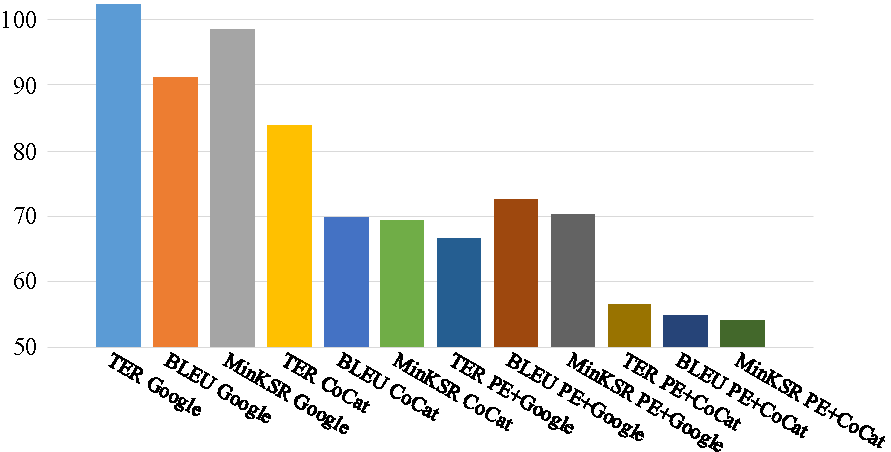
\includegraphics[width=0.85\textwidth]{Figure/Figure_3_10.pdf}
	\caption{不同评价指标之间的翻译时间比较}
	\label{Fig_metric_time}
\end{figure}

\begin{figure}[!htb]
	\centering
	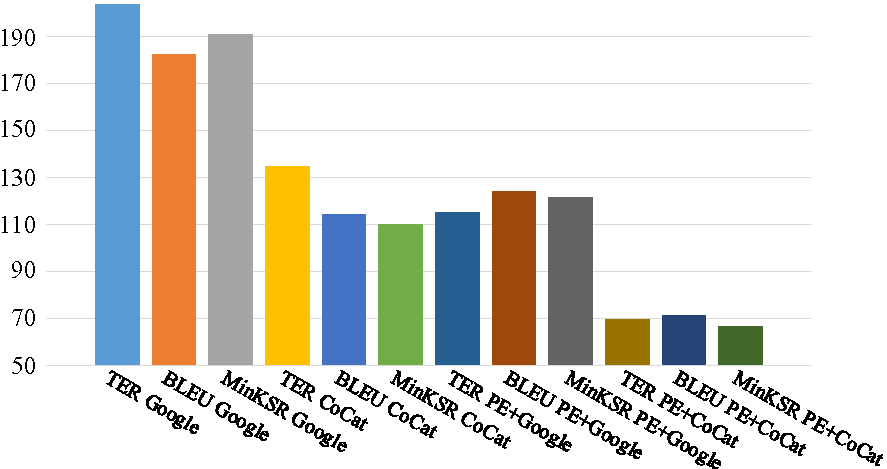
\includegraphics[width=0.85\textwidth]{Figure/Figure_3_11.pdf}
	\caption{不同评价指标之间的按键数比较}
	\label{Fig_metric_keysroke}
\end{figure}

\begin{figure}[!htb]
	\centering
	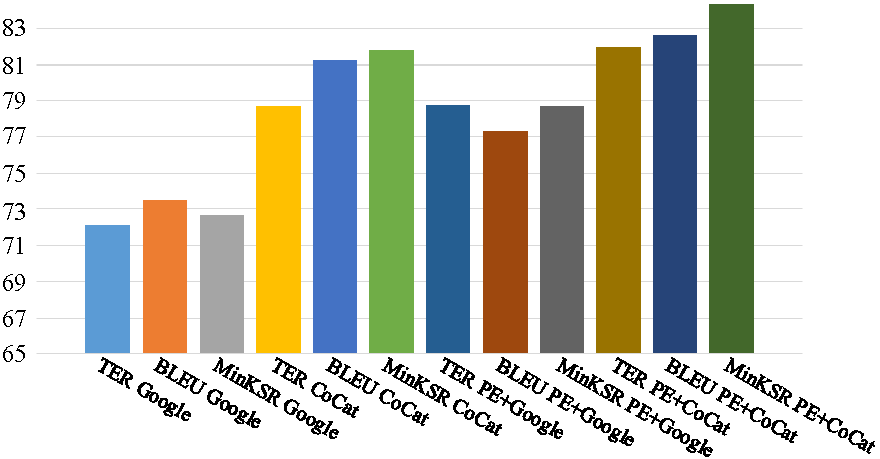
\includegraphics[width=0.85\textwidth]{Figure/Figure_3_12.pdf}
	\caption{不同评价指标之间的人工翻译质量(BLEU值)比较}
	\label{Fig_metric_quality}
\end{figure}

结合表\ref{Table_metric_compare}和\ref{Table_practical_keystroke}中的数据,我们可以发现,如果分别用MinKSR、BLEU与TER进行机器翻译的最小错误率训练,测试集上的MinKSR得分与实际按键节省率确实是正相关的。同时再次验证,MinKSR的行为与BLEU非常类似,但在实际按键数方面,MinKSR更有优势。这主要是因为MinKSR分值衡量的是按键节省率的理论下界,所以实际的按键节省率更能反映出二者的区别。

\textbf{(2.3)人工翻译测试}

最后,我们进行人工翻译实验来评估不同的译文自动评价指标对使用CoCat 输入法的人工翻译效率的影响。除机器翻译系统最小错误率训练时所用的译文自动评价指标和测试数据外,本次测试与前文中的输入法测试的实验设置完全一样。前文中的输入法测试的译文自动评价指标为TER。因此,本次人工翻译测试需要评估的是BLEU和MinKSR。测试数据分布情况如表\ref{Table_minksr_test_set}所示。综合表\ref{Table_minksr_time_keystroke_quality}的数据,完整的人工翻译测试的实验结果数据见表\ref{Table_compare_merics}。“**”表示比基线系统在置信区间$p<0.01$显著提高。

表\ref{Table_compare_merics}中,为简洁起见,我们省略了如表\ref{Table_minksr_time_keystroke_quality}中括号内的中间数据,同时将不同评价指标之间的翻译时间、按键数和翻译质量的比较分别放在图\ref{Fig_metric_time}、图\ref{Fig_metric_keysroke}和图3.12中。从表\ref{Table_compare_merics}中我们可以看到,就整体平均而言,无论是否启用译后编辑的翻译模式,译员使用MinKSR与CoCat输入法的组合均能通过更少的按键数更快完成翻译任务,同时达到更好的翻译质量。因此,表\ref{Table_compare_merics}中的结果进一步证实了将MinKSR作为专门面向输入方法的机器翻译译文自动评价指标是现实可行的。

就翻译时间和按键数而言,表\ref{Table_compare_merics}中的粗体数字、图\ref{Fig_metric_time}和图\ref{Fig_metric_keysroke}表明MinKSR总是显著地提高了使用CoCat输入法的译员的翻译效率,与较强的基线系统相比,节省了超过1.59\%的翻译时间和超过4.85\%的按键数。比较的数据基于行“MinKSR PE+CoCat”与行“BLEU PE+CoCat”,以及行“MinKSR PE+CoCat”与行“TER PE+CoCat”的比较。

就人工翻译质量而言,表\ref{Table_compare_merics}中的粗体数字和图\ref{Fig_metric_quality}表明MinKSR也总是显著地提高了使用CoCat输入法的译员的人工翻译质量,与较强的基线系统“BLEU PE+CoCat”相比,提高的人工译文BLEU值超过1.6个绝对百分点。

通过人工翻译测试,由以上的数据分析,我们可以知道,MinKSR确实能提高使用CoCat输入法的翻译效率。

综上所述,上述所有实验的数据结果都是有乐观前景的。在MinKSR的指导下,统计机器翻译系统能生成更多有利于辅助翻译输入法CoCat的结果。从而在人机交互式机器翻译场景中,MinKSR帮助CoCat输入法持续且稳定地减少人工翻译过程中的按键数,最后达到了显著提高实际的人工翻译效率的目的。

\section{本章小结}

在本章中,我们提出了一种新的人机交互式机器翻译的人机交互方法——面向计算机辅助翻译的中文输入方法。该输入方法能充分融合统计翻译中的翻译规则、翻译假设列表和翻译结果候选列表等相关信息, 只需较少的按键次数就可以生成准确的译文结果。一方面,该输入方法的短语生成模型通过融合统计翻译中间结果,利用较少的按键就能生成准确的输入结果。另一方面,该输入方法的N元文法提示模型根据翻译结果候选列表生成译文提示,使译员更方便地选择统计翻译的高质量片断。此外,为了指导统计机器翻译系统为译员生成更适合输入方法的翻译结果,我们提出了面向输入方法的译文自动评价指标,用于统计机器翻译系统的最小错误率训练。人工翻译实验结果表明,该输入方法能大幅减少翻译人员的译文修改强度,显著提高翻译效率和译文质量。同时,我们提出的输入方法还可以与译后编辑结合以进一步提高翻译效率。